In this chapter we will build a meta-population system consisting of islands connected by migration. On each island there are two populations: foxes and rabbits. The purpose of this exercise is to show how you can create many similar boxes (the islands), and how boxes (the sub-populations on islands) can be connected dynamically in \CPP\ code.

In this model, for simplicity, the foxes and rabbits do not interact. All sub-populations simply die out while connected through migration. To let foxes eat rabbits and let the animals reproduce is left as an exercise to the reader.

The box scripts rely on three box classes: \code{Island}, \code{Migration} and \code{Population}. Their \CPP\ implementation can be found in the \filename{src/plugins/demo} of your downloaded source code (see \iref{ch:build-us}).

\section {Random initial condititions}
We will start out with a single island inhabited by foxes and rabbits. The classes \code{Island} and \code{Population} are very simple; they only define a few inputs and add no functionality of their own. Here is the box script the uses them:
\lstset{numbers=left}
\begin{boxscript}
// book/demo/migration/islands-1.box
Simulation sim {
	.iterations = 3
	.steps = 1
	demo::Island island {
		.latitude = ./random/latitude[value]
		.longitude = ./random/longitude[value]
		Box random {
			RandomUniform latitude {
				.minValue = 10
				.maxValue = 20 
				.drawAtInitialize = TRUE
			}
			RandomUniform longitude {
				.minValue = -40
				.maxValue = -30
				.drawAtInitialize = TRUE
			}
		}
		demo::Population fox {
			Stage fox {
				.initial = ./random[value]
				.duration = 12
				RandomUniform random {
					.minValue = 1
					.maxValue = 100 
					.drawAtReset = TRUE
				}
			}
		}
		demo::Population rabbit {
			Stage rabbit {
				.initial = ./random[value]
				.duration = 4
				RandomPoisson random {
					.mean = 100
					.drawAtReset = TRUE
				}
			}
		} 
	} // island
	OutputR {
		PageR {
			PlotR {
				.ports = (*[latitude] *[longitude])
			}
			PlotR {
				.ports = ( *[initial]*[outflowTotal])
			}
		}
	}
}
\end{boxscript}
\lstset{numbers=none}

The \code{latitude} and \code{longitude} inputs of the \code{island} (lines 6-7) are set to random values generated inside the intervals $[10;20[$ and $[-40;-30[$ (lines 9-18), respectively. Initial population densities (lines 22 and 33) are likewise randomly generated (lines 24-28 and 35-38). Just for demonstration the initial rabbit population is drawn from a Poisson distribution (lines 35-38).

The simulation has been set to run only one time step (line 4) for three iterations (line 3). This way we can better focus on getting the structure of the model right.

Here we have run the model to study the output at the R prompt (\code{fox.initial} column not shown) :
\begin{rdialog} 
> sim
  iteration step latitude longitude rabbit.initial
1         1    0  19.1574  -33.6024            107
2         1    1  19.1574  -33.6024            107
3         2    0  19.1574  -33.6024            101
4         2    1  19.1574  -33.6024            101
5         3    0  19.1574  -33.6024             95
6         3    1  19.1574  -33.6024             95
\end{rdialog} 

The meaning of the flags \code{drawAtInitialize} (lines 12 and 17) and \code{drawAtReset} (lines 27 and 37) now becomes apparent: The position of the island is drawn only once (in the \concept{initialize} step), while the initial population densities are drawn in the \concept{reset} step of every iteration. You may want to review the \concept{computation steps} of \US\ in \iref{ch:computations}.

If you replace \code{drawAtInitialize} with \code{drawAtReset}, you will see that the island now gets a new position for every iteration. Depending on the purpose of the simulation, this could make sense as well.

\section{Cloning a box: true copies}
Above we created three islands in a row but they existed only in one copy at a time; in every iteration of the simulation, only one \code{island} box existed. However, we can use \code{island} as a template, from which to create as many clones (\ie\ copies) as we like, by putting it inside a \code{Maker} box. Here we are creating three \code{Island} boxes. They will all become child boxes of the \code{Maker} box which we have called \code{islands} (another meaningful name would have been \code{archipelago}):
\lstset{numbers=left}
\begin{boxscript}
// book/demo/migration/islands-2.box (abbreviated)
Simulation sim {
	.iterations = 3
	.steps = 1
	Maker islands {
		.replicates = 3
		demo::Island island {
		:
		}
	}
	OutputR {
	:
	}
}
\end{boxscript}
\lstset{numbers=none}

The number of clones to make is set by the \code{Maker}'s \code{replicates} input (line 6). When we study the output from the simulation (not shown), we see that \code{island} was used to clone three copies, named \code{island0}, \code{island1} and \code{island2}; there is no box called \code{island}. The islands have different locations but in each iteration, all populations start out with new initial numbers.

To get an overview of all the boxes created by a box script, whether explicit or implicit, you can type the \uscom{write} command at the \US\ prompt after loading the box script. This will write a new box script to your hard drive with a complete inventory of all the boxes currently loaded into \US, including a complete list of the inputs and outputs for each box. For convenience, the extended command \uscom{write edit} will open the generated box script for you in the text editor. Here you can verify that, in fact, the \code{island} box was cloned three times:
\lstset{numbers=left}
\begin{boxscript}
// Box script generated by 'write edit' (abbreviated)
Simulation sim{
  .iterations = 3
  .steps = 1
	:
  Maker islands{
    .replicates = 3
    .names = (island0 island1 island2)
    .fileName = ""
    demo::Island island0{ //amended
		:
    }
    demo::Island island1{ //amended
		:
    }
    demo::Island island2{ //amended
		:
		}
  }
  OutputR {
	:
  }
}
\end{boxscript}
\lstset{numbers=none}

The clones above are all true copies of the original template. Their ultimate differences were caused by their random inputs. 

\section{Cloning a box: specific copies}
Quite often you would like the cloned copies to be mostly identical but differ specifically in a few of their input values. For this purpose we create a tab-separated text file and supply it as input to \code{Maker}; each line will result in one copy being produced. Each column holds the input values specific to each clone produced:
\begin{boxscript}
// book/demo/migration/islands-3-setup.txt
.[names]	island[latitude]	island[longitude]
NewHaven	5.5	20.2
Exotica	8.2	25.9
Lampedusa	12.3	17.0
\end{boxscript}

The \code{.[names]} column is optional. It can be used to set the name of each clone which will otherwise simply be numbered. The other columns are headed by a label which must specify an input belongin to the clone or on of the boxes that it holds. In this example, values for the \code{latitude} and \code{longitude} inputs to \code{island} are given. 

You hand this text file to the \code{Maker} box through its \code{fileName} input. The \code{Maker} will itself find out how many clones to produce from the file, so you do not set the \code{iterations} input as above. Here it is
\lstset{numbers=left}
\begin{boxscript}
// book/demo/migration/islands-3.box (abbreviated)
Simulation sim {
	.iterations = 3
	.steps = 30
	Maker islands {
		.fileName = "islands-3-setup.txt"
		demo::Island island {
		:
		}
	}
	OutputR {
	:
	}
}
\end{boxscript}
\lstset{numbers=none}

If you load this box script and then type \uscom{write edit}, you can check that three island boxes have been created with the given names and geographical locations.

\section{Coding a mediator class: Migration}
What is missing from our model is the most complicated part, namely the migration process. It turns out that box scripts by themselves are not expressive enough to formulate the logic of migration. To model migration we need to set up  input-output relations between between all sub-populations depending on some measure of connectedness, which might itself change dynamically.

The \code{Migration} class (found in the \code{demo} plug-in) solves this problem through intricate manipulations of the boxes in the script: the \code{Island} boxes inside the \code{Maker} parent box, the \code{Population}s inside each \code{Island}, and even the \code{Stage} inside each \code{Population}. 

Classes, such as \code{Migration} that interfere deeply with other objects are called \concept{mediator} classes. They tend to be complex and sensitive to code changes outside themselves because they interact with and make assumptions about details of code and structure outside the mediator class itself.

For this reason, one tries to avoid mediator classes, or if their service is needed, to have as few of them as possible; preferentially, just one. Here we need a mediator class, and we call it \code{Migration}.

The ease, with which the \code{Migration} box is used, belies its internal complexity; we simply add it to the previous box script:
\lstset{numbers=left}
\begin{boxscript}
// book/demo/migration/islands-4.box (abbreviated)
Simulation sim {
	.iterations = 3
	.steps = 30
	Maker islands {
		.fileName = "islands-3-setup.txt"
		demo::Island island {
		:
		}
	}
	Maker migration {
		.names = (fox rabbit)
		demo::Migration  {
		}
	}
	OutputR {
	:
	}
}
\end{boxscript}
\lstset{numbers=none}

Except for lines 11-15 nothing else has changed. Here we are using the third and last way of determining how \code{Maker} performs the cloning: By specifying a vector of names to the \code{names} input, identical copies will be produced and given the names supplied in the vector (line 12). In this case, two \code{Migration} boxes, named \code{fox} and \code{rabbit}, will be produced. The names of the \code{Migration} boxes must match the names of the populations on the islands, as will be evident in the \CPP\ code.

Before walking through the \CPP\ code for the \code{Migration} class, let's get an overview how it sets up the input-output pathways between itself and the populations that it acts upon. First load the \filename{islands-4.box} script and then issue the \uscom{write edit} command. Leaf through the generated box script in the editor and find the two \code{Migration} boxes called \code{fox} and \code{rabbit}:

\lstset{numbers=left}
\begin{boxscript}
// Box script generated by 'write edit' (excerpt)
Maker migration{
	.replicates = 2
	.names = (fox rabbit)
	.fileName = ""
	demo::Migration fox{ //amended
		//>em0 == 0
		//>im0 == ()
		//>em1 == 0
		//>im1 == ()
		//>em2 == 0
		//>im2 == ()
	}
	demo::Migration rabbit{ //amended
		//>em0 == 0
		//>im0 == ()
		//>em1 == 0
		//>im1 == ()
		//>em2 == 0
		//>im2 == ()
	}
}
\end{boxscript}
\lstset{numbers=none}

As noted by the comments in the script above, the box script was amended with the boxes \code{fox} and \code{rabbit} (lines 6 and 14). These amendments were carried out by the \code{Maker} box (line 2). The addition of output ports (lines 7-12 and 15-20), however, was an amendment caused by each \code{Migration} box on its own, based on the populations found on the islands. 

For each population found, \code{Migration} creates an emigration and immigration output (\eg\ lines 7-8). The immigration output is a vector, yet empty, because we just loaded the box script but did yet run it. To keep the outputs separate for each population, they are enumerated 0, 1, \ldots

Further up in the generated box script, you can find where the outputs of the \code{Migration} boxes are set as inputs to the \code{Stage} boxes, that hold the foxes and rabbits. For example, for the first \code{Island} box named \code{NewHaven}, you will find that the \code{phaseInflow} and \code{phaseOutflowProportion} inputs have been set to the corresponding outputs of the \code{Migration} boxes: 
\lstset{numbers=left}
\begin{boxscript}
// Box script generated by 'write edit' (excerpt)
demo::Island NewHaven{ //amended
	.latitude = 5.5
	.longitude = 20.2
	demo::Population fox{ //amended
		.emigrationSlope = 4
		Stage fox{ //amended
			.k = 30
			.duration = 12
			:
			.phaseInflow = /sim/migration/fox[im0]
			:
			.phaseOutflowProportion = /sim/migration/fox[em0]
			:
		}
		Stage rabbit{ //amended
			.k = 30
			.duration = 4
			:
			.phaseInflow = /sim/migration/rabbit[im0]
			:
			.phaseOutflowProportion = /sim/migration/rabbit[em0]
			:
		}
	}
}
\end{boxscript}
\lstset{numbers=none}

Note that these inputs were not set in the original box script; there were set by the \CPP\ code of the \code{Migration} class, as we shall soon see.

To understand how immigration and emigration is applied to a \code{Stage} box, one must realise that the content of a \code{Stage} is held in a vector, representing an age-distributed population (\iref{fig:stage}). In one end, young individuals enter as an inflow set by the \code{inflow} input, while at the other end old individuals exit as given by the \code{outflow} output. The course of this development is determined by several other parameters provided as inputs: \code{duration}, \code{k}, \code{growthRate} and \code{timeStep}. The latter two can be time-varying.

Some biological processes (emigration, infection, parasitization and predation) can be modelled, as if a slice of the vector is cut away. This is governed by the \code{phaseOutputProportion} input which causes a proportional reduction of all elements in the vector. The resulting slice is given by the \code{phaseOutflow} vector.

While the \code{phaseOutflow} output is always proportional to the current content of the age-distributed vector, the \code{phaseInflow} vector can hold any distribution. 

When a \code{Stage} box is updated, first the \code{inflow} is added to the first age class, and the \code{phaseInflow} is added by vector addition across age classes. Then the vector is updated to produce the \code{outflow} and \code{phaseOutflow} outputs.

\begin{figure} [hb]
\centering
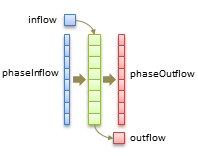
\includegraphics[scale=1]{graphics/stage}
\caption{Flows in (blue) and out (red) of a \code{Stage} box. The age-distributed content of the \code{Stage} is kept in a vector (green).}
\label{fig:stage}
\end{figure}

The \code{Migration} header file (next page) sets up data structures to hold the information needed to compute all island-to-island migrations rates.

\begin{figure}
\centering
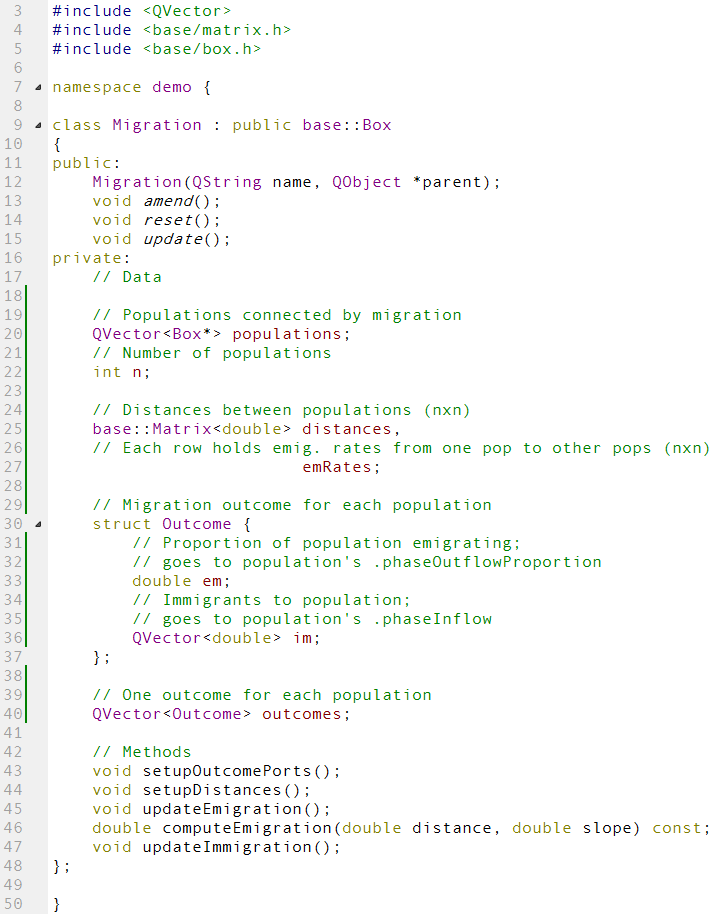
\includegraphics[scale=0.7,left]{graphics/migration-h}
\end{figure}

Firstly, header files to allow the use of vectors and matrices are included (lines 3-4). Header files preceded by \code{base} belong to the base library of \US. A vector of pointers to \code{Box} objects is held in \code{populations} (line 20). For convenience, \code{n} is set to the length of the vector. 

A matrix hold distances between all populations (line 25). In our case, it will be symmetrical (for other organisms an asymmetric matrix could result, \eg\ from a prevailing wind direction). Another matrix (line 26) holds the emigration rates. Each row represents the emigration from one population to all the other populations. The row includes the population itself for which the emigration rate will be zero.

The realised migration rates, which will be updated for every time step, are held in a structure (lines 30-37) with two members: \code{em} which is the proportion leaving the population and \code{im} which is a vector of immigrants entering the population. 

The \code{Outcome} structure is declared in lines 30-37. In line 40 is it used as a component in a larger data structure: \code{outcomes} is a vector holding an \code{Outcome} structure for each population, \ie\ each population has one number representing the proportional loss to emigraton (\code{em}) and one vector (\code{im}) representing the age-distributed immigration.

The \code{amend} method first finds all the populations present in the box script (lines 18-19). Recall that the name of the \code{Migration} object will be either \code{fox} or \code{rabbit}, as declared in the box script. The \code{name()} method is used to retrieve the object name (line 18), giving \code{popPath} a value of, \eg\ \code{"islands/*/fox"}. Subsequently (line 19), we apply \code{findMany<Box>}, as it returns a vector of pointers to the \code{Box} objects matching the path given as its argument.

\begin{figure} [ht]
\centering
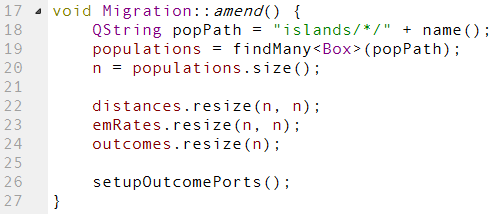
\includegraphics[scale=0.7,left]{graphics/migration-cpp-amend}
\end{figure}

The sizes of vector and matrix data structures are set according to the number of populations found (lines 20-24). Finally, \code{setupOutcomePorts} is called to add the necessary output ports for the emigration and immigration rates of all populations.

\begin{figure} [ht]
\centering
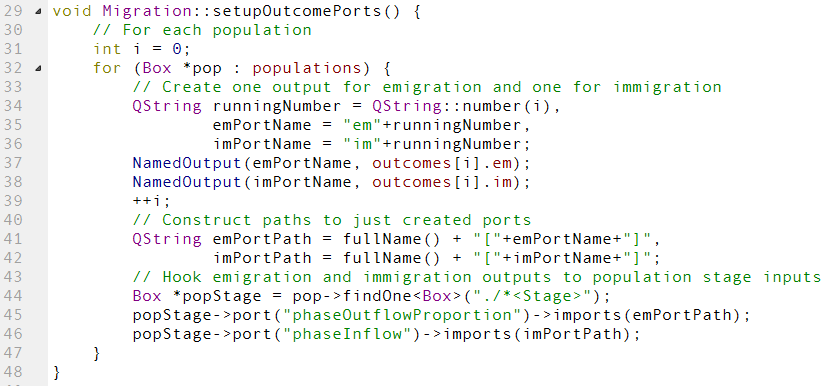
\includegraphics[scale=0.7,left]{graphics/migration-cpp-setup-outcome-ports}
\end{figure}

For each population we first construct names for the ports to be added (lines 34-36), \ie\ \code{emPortName} and \code{imPortName} will be \code{"em0"} and \code{"im0"}, respectively, first time around.

These names are then assigned to two new output ports created by \code{NamedOutput}, which takes two arguments: first the name of the output port and second the variable which holds the value of the output port (lines 37-38). Note how index \code{i} is used to find the proper structure in the \code{outcomes} vector.

After the two output ports have been created we must link the proper input ports to them. First we construct the paths to the output ports. The \code{fullName} method returns the path all the way from the root, so we get \eg\ for \code{emPortPath} the value \code{"/sim/migration[em0]"} (line 41).

Next we find the \code{Stage} box that the \code{Population} box holds inside as a child box. We ask the population to find exactly one box matching the path \code{"./*<Stage>"} (line 44). Literally, this path expression means 'in me find a child of any name of class \code{Stage} (consult \iref{us:find} for more details on path expressions).

Finally, for the found stage box (\code{popStage}) its \code{phaseOutputProportion} input is set to import (\ie\ reference) the \code{em} output, and the \code{phaseInflow} input is set to import the \code{im} output (\cf\ \iref{fig:stage}).

The \code{reset} method simply calls methods to set up up the distance matrix and to update the emigration matrix (lines 51 and 53). It also demonstrates how to send text to be displayed at the \US\ prompt through the \code{information} method accessed by \code{dialog()} (lines 52 and 54). The \code{information} method takes a string as an argument.

\begin{figure} [hb]
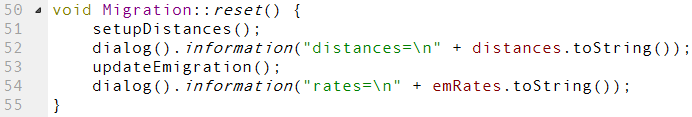
\includegraphics[scale=0.7,left]{graphics/migration-cpp-reset}
\end{figure}

The \code{setupDistances} methods cheats in using Euclidian distance on latitudes-longitudes. You can find more appropriate equations on the web. It runs through all the pairwise combinations of populations in a double for loop (lines 58-68). However, it is not the populations that carry the geographical information but their parent, which is of the \code{Island} class. We find the parents of the $i$'th and $j$'th populations (lines 60-61) using the double-dot (\code{".."}) path (\cf\ \iref{us:find}). Pointers to the parents we find are kept in \code{island1} and \code{island2}.

If you have a pointer to a \code{Box} object and want to access one of its ports, you use the \code{port} method, which takes the port name as an argument (lines 62-65). The \code{port} method returns a pointer to a \code{Port} object. 

A port could hold many kinds of values. To retrieve the value, you use the \code{value} method specifying which type of value you want through its so-called \concept{template parameter}, \eg\ you write \code{value<double>()} to retrieve the port value as a double-precision floating point number. Besides the template parameter, the \code{value} method takes no arguments.

The calculated distance is stored in the \code{distances} matrix (line 66). Note that you cannot use brackets to index into a matrix, as you can for vectors. You must use parentheses.

\begin{figure} [ht]
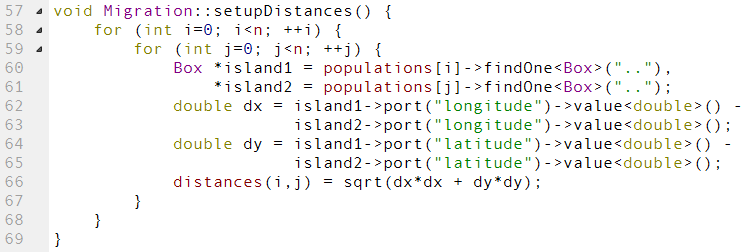
\includegraphics[scale=0.7,left]{graphics/migration-cpp-setup-distances}
\end{figure}

\begin{figure} [b]
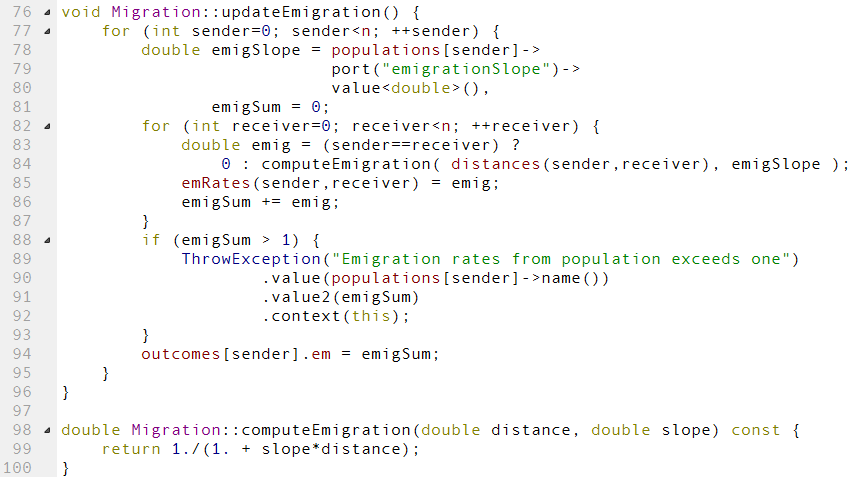
\includegraphics[scale=0.7,left]{graphics/migration-cpp-update-emigration}
\end{figure}

The \code{updateEmigration} function goes through the \code{distances} matrix in a double-loop (lines 77-95). The outcome of the calculation is a proportional emigration rate $[0;1]$ for each population, which is accumulated for every \code{sender} population over all \code{receiver} populations inside the inner loop (line 86).

The emigration rate for every \code{receiver} is computed using the \code{computeEmigration} method which, admittedly, is rather primitive; it does not even secure that the total emigration does not exceed 100\%. Hence, this needs to be tested (lines 88-93). 

The call of \code{ThrowException} will cause the simulation run to stop with the given error message. Optional information can be given, glued on by dot notation. As exemplified here, \code{value} and \code{value2} can be used to display common value types, \eg\ strings (line 90) and numbers (line 91). The \code{context} method is passed a pointer to the current object, which will help to locate the error.

The emigration rate depends on the distance between the populations, which we get from the \code{distances} matrix (line 84), and also on \code{emigrationSlope} which is an input to the \code{Population} box. For every \code{sender}, we retrieve the current value of \code{emigrationSlope}, which is currently fixed in the model but could be made \eg\ density-dependent later on, and store it in the \code{emigSlope} variable (lines 78-80).

Finally, for every \code{sender} the accumuluated emigration rate is stored in the proper place in the \code{outcomes} vector (line 94). Note that, we have already (in \code{setupOutputPorts}) arranged that all \code{outcomes[i].em} are linked to the appropriate input ports in the sender's \code{Stage} box.

For the \code{update} method there is nothing to do but updating the emigration and immigration outcomes (lines 72-73).

\begin{figure} [ht]
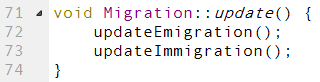
\includegraphics[scale=0.7,left]{graphics/migration-cpp-update}
\end{figure}

Before studying the code of the \code{updateImmigration} method, we must realise that at this point, all \code{Stage} boxes have had their \code{phaseOutflow} output calculated (\iref{fig:stage}). These outflows represent the material that we must now divide between the receiving stages, each receiving stage receiving material from all the other, sending stages.

To ease the reading, we create a type \code{Cohorts} as a short-hand for a vector of floating-point numbers (line 104). Then for every sending population, we find its \code{Stage} box (line 107) by which we retrieve the cohorts in its \code{phaseOutflow} output and store them in the \code{emig} variable (line 108).

We are now ready to split these emigrants among the receiving populations. The \code{proportionReceived} by each receiver is proportional to the emigration rate to that particular receiver from the sender divided by the sum of all emigrations rates from the sender (lines 111-112).

Mathematically, we need to carry out the following summation,

$outcomes[receiver].\overline{im} = \sum\limits_{receiver=0}^{n-1} \overline{emig} * proportionReceived$,
but neither multiplication nor summation can be expressed directly on a \code{QVector} variable. The \code{vector_op} namespace contains a set of functions for various \code{QVector} operations. You can find them in the \filename{vector_op.h} header file in the \code{base} plug-in. Here we will use two of these functions, listed in the header file as
\begin{cpp}
void product(Vec &v, const Vec &x, const Scalar &y);
void add(Vec &v, const Vec &x, QObject *context=0);
\end{cpp}

The functions carry out these operations, respectively, $\overline{v} \leftarrow \overline{x} y$ and $\overline{v} \leftarrow \overline{v} + \overline{x}$.

In the header file, \code{Vec} is a shorthand for \code{QVector<double>} and \code{Scalar} is a stand-in for \code{double}. In all these functions, arguments qualified by \code{const} are inputs to the function, while those without will receive the result of the calculation. The optional \code{context} argument in some functions will be used in case of error (\ie\ non-matching vector dimensions).

\begin{figure} [ht]
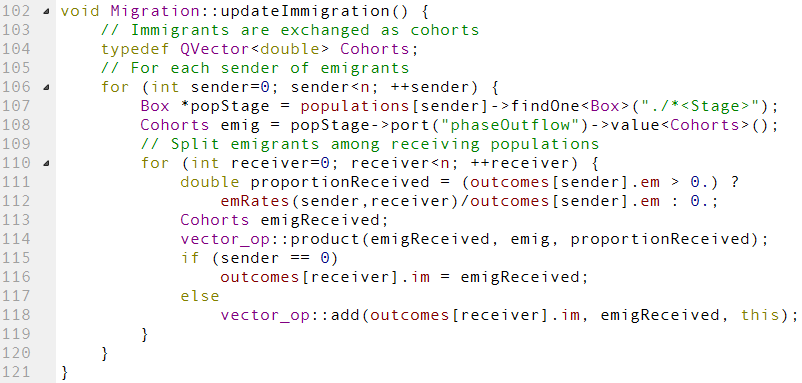
\includegraphics[scale=0.7,left]{graphics/migration-cpp-update-immigration}
\end{figure}

In the code, we store the proportion of emigrants received in the \code{emigReceived} vector (lines 113-114). First time around (when \code{sender} equals zero), we simply put the emigrants received into the proper \code{receiver} in the \code{outcomes} vector (lines 115-116). Subsequently, we accumulate the emigrants in the same place (line 118).

In the end, the \code{outcomes} vector have been updated with the accumulated vectors of immigrants received by each population. This will end up in the proper \code{Stage} boxes, as we already (in \code{setupOutputPorts}) linked these immigrant vectors to \code{Migration} output ports and put them as \code{phaseInflow} to the stages (\cf\ \iref{fig:stage}).

